%  LaTeX support: latex@mdpi.com
%  For support, please attach all files needed for compiling as well as the log file, and specify your operating system, LaTeX version, and LaTeX editor.

%=================================================================
\documentclass[hydrology,article,submit,pdftex,moreauthors]{Definitions/mdpi}

% Additional packages
\usepackage{listings}
\usepackage{longtable}

% Code listing style
\lstset{
  basicstyle=\ttfamily\small,
  breaklines=true,
  frame=single,
  language=Python,
  numbers=left,
  numberstyle=\tiny\color{gray},
  keywordstyle=\color{blue},
  commentstyle=\color{green!50!black},
  stringstyle=\color{red!70!black},
  showstringspaces=false,
  xleftmargin=2em,
  framexleftmargin=1.5em
}

%=================================================================
% MDPI internal commands - do not modify
\firstpage{1}
\makeatletter
\setcounter{page}{\@firstpage}
\makeatother
\pubvolume{1}
\issuenum{1}
\articlenumber{0}
\pubyear{2026}
\copyrightyear{2026}
%\externaleditor{Academic Editor: Firstname Lastname}
\datereceived{ }
\daterevised{ }
\dateaccepted{ }
\datepublished{ }
\hreflink{https://doi.org/}

%=================================================================
% Full title of the paper (Capitalized)
\Title{A literature review of baseflow separation algorithms and an accompanying computational package}

% MDPI internal command: Title for citation in the left column
\TitleCitation{A Literature Review of Baseflow Separation Algorithms and an Accompanying Computational Package}

% Author ORCID IDs
\newcommand{\orcidauthorA}{0000-0002-7597-2825} % Norman Jones

% Authors, for the paper (add full first names)
\Author{Xueyi Li~$^{1}$, Amin Aghababaei~$^{1}$, Ryan van der Heijden~$^{2}$, Eniola Webster-Esho~$^{3}$, Joshua Hart~$^{1}$, Amber Kunz~$^{1}$, Berkeley Berrett~$^{1}$, Norman Jones~$^{1,}$*\orcidA{}, Gus Williams~$^{1}$, Donna Rizzo~$^{2}$, and T.~Prabhakar Clement~$^{3}$}

% MDPI internal command: Authors, for metadata in PDF
\AuthorNames{Xueyi Li, Amin Aghababaei, Ryan van der Heijden, Eniola Webster-Esho, Joshua Hart, Amber Kunz, Berkeley Berrett, Norman Jones, Gus Williams, Donna Rizzo and T. Prabhakar Clement}

% MDPI internal command: Authors, for citation in the left column
\AuthorCitation{Li, X.; Aghababaei, A.; van der Heijden, R.; Webster-Esho, E.; Hart, J.; Kunz, A.; Berrett, B.; Jones, N.; Williams, G.; Rizzo, D.; Clement, T.P.}

% Affiliations / Addresses
\address{%
$^{1}$ \quad Civil and Construction Engineering, Brigham Young University, Provo, UT 84602, USA\\
$^{2}$ \quad Civil and Environmental Engineering, University of Vermont, Burlington, VT 05405, USA\\
$^{3}$ \quad Civil, Construction and Environmental Engineering, University of Alabama, Tuscaloosa, AL 35487, USA}

% Contact information of the corresponding author
\corres{Correspondence: njones@byu.edu; Tel.: +1-801-225-0799 (N.J.)}

%\simplesumm{}

%\conference{}

% Abstract (Do not insert blank lines, i.e. \\)
\abstract{Baseflow, the portion of streamflow sustained by groundwater discharge, is fundamental to watershed hydrology, water resource management, and ecological assessment. Because baseflow cannot be measured directly, it must be estimated by separating it from total streamflow, and decades of research have produced a large and diverse collection of separation methods. This paper presents a review of these methods, organizing them into four methodological paradigms: recursive digital filters, graphical hydrograph-partitioning methods, recession-based methods, and tracer-based approaches. Within the recursive digital filter paradigm, we show that the many filters proposed by different authors can be expressed as special cases of a single generalized three-parameter equation, which exposes the algebraic relationships among popular methods and separates them into linear-reservoir and signal-processing families. For each paradigm we discuss the underlying assumptions, parameter requirements, and practical trade-offs that guide method selection. To make these methods readily accessible and directly comparable, we also describe \texttt{baseflowx}, an open-source Python package that implements 17 of the reviewed methods behind a consistent interface, together with built-in USGS data retrieval and a conductivity mass balance (CMB) module that links tracer measurements to digital-filter parameters. We further present the Baseflow Explorer, a companion web application that makes all separation methods accessible through an interactive map-based interface without requiring Python expertise, enabling on-demand analysis of approximately 9{,}500 active USGS stream gages across the contiguous United States. Together, the package and web application provide a unified platform for applying and comparing baseflow separation methods that have historically been scattered across legacy programs, web tools, and research scripts.}

% Keywords
\keyword{baseflow separation; digital filter; Python; open-source software; recession analysis; streamflow; tracer; hydrology}

%%%%%%%%%%%%%%%%%%%%%%%%%%%%%%%%%%%%%%%%%%
\begin{document}

%%%%%%%%%%%%%%%%%%%%%%%%%%%%%%%%%%%%%%%%%%
\section{Introduction}
\label{sec:introduction}

Streamflow comprises two primary components: quickflow, which responds rapidly to precipitation and snowmelt events, and baseflow, which represents the slower, sustained contribution from groundwater discharge, bank storage, and other delayed sources. The relative contribution of baseflow to total streamflow is commonly quantified by the baseflow index (BFI), defined as the ratio of cumulative baseflow volume to cumulative total streamflow volume over a given period ($\mathrm{BFI} = \sum b_t / \sum Q_t$); values close to 1 indicate groundwater-dominated catchments, while values close to 0 indicate flashy, quickflow-dominated catchments. Baseflow is critical for sustaining river ecosystems during dry periods~\cite{Smakhtin2001}, supporting water supply planning, managing groundwater--surface water interactions~\cite{Barlow2012}, and calibrating hydrological models~\cite{ChapmanMaxwell1996,Eckhardt2005}. As climate and land-use change continue to alter the global water cycle, understanding baseflow dynamics has become increasingly important~\cite{Tan2020,Jasechko2024}. However, baseflow cannot be measured directly in the field~\cite{ChapmanMaxwell1996}, so practitioners rely on separation methods to estimate it from observed total streamflow records.

Over several decades, a diverse array of separation methods has been developed, as summarized in several reviews~\cite{Tallaksen1995,McMahon2021}. These methods can be broadly organized into four categories. \textit{Recursive digital filters} apply signal-processing or linear-reservoir-based equations to partition the hydrograph into baseflow and quickflow components~\cite{Lyne1979,Nathan1990,Chapman1991,Eckhardt2005}. \textit{Graphical methods} identify baseflow through geometric rules applied to the hydrograph, such as fixed intervals, sliding windows, or local minima~\cite{Sloto1996}. \textit{Recession-based methods} exploit the characteristic exponential decay of baseflow during dry periods to anchor separation points~\cite{Tallaksen1995,Rutledge1998}. \textit{Tracer-based methods} use hydrochemical measurements, such as specific conductance or stable isotopes, to quantify the groundwater fraction via mass balance~\cite{Stewart2007,Klaus2013}. The choice of method can substantially affect the resulting baseflow index, as demonstrated by comparative studies across diverse catchments~\cite{Eckhardt2008,Lott2016}.

Despite the abundance of methods, practitioners face practical barriers to applying them. The U.S.\ Geological Survey (USGS) programs HYSEP (HYdrograph SEParation program;~\cite{Sloto1996}) and PART (Partitioning Antecedent Recession Trends;~\cite{Rutledge1998}) are written in legacy Fortran and are difficult to integrate into modern analytical workflows. The Web-based Hydrograph Analysis Tool (WHAT)~\cite{Lim2005} provides a graphical interface but cannot be scripted or automated. Several R packages exist but are limited to a small subset of methods~\cite{PelletierR2020}. The Python package by Xie et al.~\cite{Xie2020} implemented 11 digital filters but was designed primarily as research code for a specific comparative study, bundling geospatial and study-specific functionality that limited its reusability as a general-purpose library. More broadly, the growing Python ecosystem for hydrology, including packages such as Hydrostats~\cite{Roberts2018} and Pastas~\cite{Collenteur2019}, has demonstrated the value of well-documented, pip-installable tools, yet no comprehensive Python package for baseflow separation has been available.

To address these gaps, we present \texttt{baseflowx}, an open-source Python package that provides a unified, consistent interface to 17 baseflow separation methods across all four methodological paradigms, and the Baseflow Explorer, a companion web application that delivers the same methods through a browser-based map interface. The package builds on the work of Xie et al.~\cite{Xie2020} but has been extensively refactored: study-specific code has been removed, four new methods have been added (PART, CMB, IHACRES (Identification of unit Hydrographs And Component flows from Rainfall, Evaporation, and Streamflow data), and BFlow), a new tracer module has been introduced, and the recursive digital filters have been unified under a single generalized equation. The result is a focused, pip-installable library with a flat, function-oriented application programming interface (API), built-in USGS data retrieval, Numba-accelerated performance, and comprehensive documentation.

This paper is organized as follows. Section~\ref{sec:litreview} reviews the baseflow separation literature, tracing the development of the four methodological paradigms, synthesizing comparative studies, and surveying gaps in existing software. Section~\ref{sec:design} describes the architecture and implementation of \texttt{baseflowx}. Section~\ref{sec:examples} demonstrates usage through worked examples. Section~\ref{sec:validation} presents a cross-method BFI comparison across all 17 methods. Section~\ref{sec:webapp} introduces the Baseflow Explorer web application. Section~\ref{sec:discussion} discusses the unified filter framework, limitations, and future directions. Section~\ref{sec:conclusions} concludes.

%%%%%%%%%%%%%%%%%%%%%%%%%%%%%%%%%%%%%%%%%%
\section{Literature Review: Baseflow Separation Methods}
\label{sec:litreview}

\subsection{Historical Development and Context}
\label{sec:history}

Baseflow separation has a history spanning more than a century, evolving from hand-drawn hydrograph constructions to algorithmic approaches embedded in modern computational tools. Early practitioners used graphical methods to partition storm hydrographs, drawing straight lines or curves beneath the observed record to approximate the groundwater contribution~\cite{Barnes1939}. The first generation of automated methods emerged in the 1970s and 1980s: Lyne and Hollick~\cite{Lyne1979} introduced the recursive digital filter analogy from signal processing, and Nathan and McMahon~\cite{Nathan1990} systematized its application and demonstrated multi-pass variants on Australian catchments. The USGS responded with Fortran programs: HYSEP~\cite{Sloto1996} for graphical methods and PART~\cite{Rutledge1998} for recession-based separation, tools that became standard references in regulatory and water-resources practice.

A second wave of methodological development in the 2000s brought physically grounded refinements. Eckhardt~\cite{Eckhardt2005} unified the linear-reservoir filter family under a two-parameter framework parameterized by a maximum baseflow index ($\mathrm{BFI_{max}}$) that connects filter output to catchment hydrogeology. Stewart et al.~\cite{Stewart2007} demonstrated how specific conductance measurements could anchor tracer-based separation to hydrochemical data, providing an estimate independent of hydrograph shape. Subsequent work produced additional filter variants~\cite{Willems2009,Jakeman1993}, recession analysis tools~\cite{Arnold1999,Cheng2016}, and improved parameter estimation methods~\cite{Collischonn2013}. The result is a literature rich in methods but fragmented across hydrology, hydrogeology, and signal-processing communities, with implementations distributed across legacy Fortran programs, single-study Python scripts, and web tools of varying methodological breadth.

\subsection{Recursive Digital Filters}
\label{sec:generalized_filter}

A central theoretical contribution of this work is the observation that all 11 recursive digital filter methods implemented in \texttt{baseflowx} can be expressed as special cases of a single three-parameter equation:
\begin{equation}
\label{eq:generalized}
b_t = \alpha \, b_{t-1} + \beta \left( Q_t + \gamma \, Q_{t-1} \right), \quad \text{subject to} \quad b_t \leq Q_t
\end{equation}
where $b_t$ is the estimated baseflow at time $t$, $Q_t$ is the observed streamflow, and $\alpha$, $\beta$, $\gamma$ are method-specific coefficients derived from the physical or empirical parameters of each method. The constraint $b_t \leq Q_t$ ensures that baseflow never exceeds total streamflow.

The parameter $\gamma$ divides the filters into two structural families. When $\gamma = 0$, the filter depends only on the current streamflow $Q_t$ and the previous baseflow $b_{t-1}$; these filters are grounded in linear reservoir theory. When $\gamma = 1$, the filter incorporates both $Q_t$ and $Q_{t-1}$, reflecting a signal-processing origin where the moving average of streamflow is used. Table~\ref{tab:coefficients} summarizes the coefficient mappings for all recursive filters.

\begin{table}[H]
\caption{Coefficient mappings for the generalized recursive digital filter (Equation~\ref{eq:generalized}). Each named method is a special case defined by its $\alpha$, $\beta$, and $\gamma$ values.\label{tab:coefficients}}
\small
\begin{tabularx}{\textwidth}{lccccl}
\toprule
\textbf{Method} & $\boldsymbol{\alpha}$ & $\boldsymbol{\beta}$ & $\boldsymbol{\gamma}$ & \textbf{Source Parameters} & \textbf{Reference} \\
\midrule
\multicolumn{6}{l}{\textit{Family 1: Linear reservoir filters ($\gamma = 0$)}} \\
\addlinespace
Chapman--Maxwell & $\dfrac{a}{2-a}$ & $\dfrac{1-a}{2-a}$ & 0 & $a$ & \cite{ChapmanMaxwell1996} \\[6pt]
Boughton & $\dfrac{a}{1+C}$ & $\dfrac{C}{1+C}$ & 0 & $a, C$ & \cite{Boughton1993} \\[6pt]
Eckhardt & $\dfrac{(1-\mathrm{BFI_{max}})a}{1-a \cdot \mathrm{BFI_{max}}}$ & $\dfrac{(1-a)\mathrm{BFI_{max}}}{1-a \cdot \mathrm{BFI_{max}}}$ & 0 & $a, \mathrm{BFI_{max}}$ & \cite{Eckhardt2005} \\[6pt]
EWMA & $1-e$ & $e$ & 0 & $e$ & \cite{Tularam2008} \\[6pt]
Furey--Gupta & $a - A(1-a)$ & $A(1-a)$ & 0 & $a, A$ & \cite{Furey2001} \\[6pt]
WHAT & \multicolumn{4}{l}{Alias for Eckhardt~\cite{Eckhardt2005}} & \cite{Lim2005} \\
\addlinespace
\midrule
\multicolumn{6}{l}{\textit{Family 2: Signal-processing filters ($\gamma = 1$)}} \\
\addlinespace
Lyne--Hollick & $\beta_p$ & $\dfrac{1-\beta_p}{2}$ & 1 & $\beta_p$ & \cite{Lyne1979} \\[6pt]
Chapman (1991) & $\dfrac{3a-1}{3-a}$ & $\dfrac{1-a}{3-a}$ & 1 & $a$ & \cite{Chapman1991} \\[6pt]
Willems & $\dfrac{a-v}{1+v}$ & $\dfrac{v}{1+v}$ & 1 & $a, w$ & \cite{Willems2009} \\
\addlinespace
\midrule
\multicolumn{6}{l}{\textit{Hybrid: Variable $\gamma$ ($-1 < \gamma < 0$)}} \\
\addlinespace
IHACRES & $\dfrac{a}{1+C}$ & $\dfrac{C}{1+C}$ & $\alpha_s$ & $a, C, \alpha_s$ & \cite{Jakeman1993} \\
\bottomrule
\end{tabularx}
\raggedright
\footnotesize{Note: For Willems, $v = \frac{(1-w)(1-a)}{2w}$ where $w$ is the quickflow fraction. For Furey--Gupta, $\beta$ operates on $Q_{t-1}$ rather than $Q_t$ (a lagged formulation).}
\end{table}

This unification reveals several important relationships. The Eckhardt filter is algebraically equivalent to the Boughton filter under the parameter transformation $C = (1-a) \cdot \mathrm{BFI_{max}} / (1 - \mathrm{BFI_{max}})$. When $\mathrm{BFI_{max}} = 0.5$, the Eckhardt filter further reduces to the Chapman--Maxwell filter. The IHACRES filter, with its variable $\gamma = \alpha_s$ parameter, bridges the two families: when $\alpha_s = 0$ it reduces to the Boughton filter ($\gamma = 0$ family), and as $\alpha_s \to -1$ it approaches the behavior of the $\gamma = 1$ family (Figure~\ref{fig:ihacres_sensitivity}).

The multi-pass Lyne--Hollick variant~\cite{Spongberg2000} applies the single-pass filter iteratively, alternating forward and backward passes. Each additional pass further smooths the baseflow estimate and reduces the baseflow index (BFI), as illustrated in Figure~\ref{fig:lh_passes}.

\begin{figure}[H]
\centering
\includegraphics[width=0.85\textwidth]{figures/lyne_hollick_passes.png}
\caption{Effect of multiple passes of the Lyne--Hollick filter. Each additional pass produces a lower baseflow estimate and reduced BFI.\label{fig:lh_passes}}
\end{figure}

\subsubsection{Individual Recursive Filter Descriptions}
\label{sec:filter_descriptions}

The following paragraphs describe the physical interpretation and key parameters of each recursive digital filter implemented in \texttt{baseflowx}. Together with the coefficient mappings in Table~\ref{tab:coefficients}, these descriptions provide the information needed to select and interpret each method.

\paragraph{Lyne--Hollick Filter.}
The Lyne--Hollick filter~\cite{Lyne1979} was among the first recursive digital filters proposed for baseflow separation, adapting signal-processing concepts to streamflow partitioning. The single free parameter $\beta_p$ (also written $\alpha$ in some texts, and typically set between 0.90 and 0.95) controls the fraction of the previous baseflow carried forward in time; values close to unity produce smooth, slowly varying baseflow estimates with a high BFI. Nathan and McMahon~\cite{Nathan1990} systematized the application of this filter on Australian catchments and recommended the three-pass variant, in which the single-pass filter is applied forward and then backward (and forward again) to eliminate phase shift introduced by the one-directional recursion. The single-pass filter tends to produce a relatively high BFI (0.74 for the Fish River example in this paper), while each additional pass progressively reduces the estimate by removing higher-frequency components of the signal.

\paragraph{Chapman (1991) Filter.}
Chapman~\cite{Chapman1991} proposed a modification to the Lyne--Hollick formulation that introduces the recession coefficient $a$ as the sole parameter, thereby linking the filter to the physically interpretable groundwater recession time scale rather than an empirically chosen signal-processing constant. The filter coefficients $\alpha = (3a-1)/(3-a)$ and $\beta = (1-a)/(3-a)$ are uniquely determined by $a$, which can be estimated directly from the streamflow record using recession analysis. This grounding in linear reservoir theory makes the Chapman filter a parsimonious bridge between the signal-processing ($\gamma = 1$) and physically based filter traditions.

\paragraph{Chapman--Maxwell Filter.}
Chapman and Maxwell~\cite{ChapmanMaxwell1996} introduced a filter within the linear-reservoir ($\gamma = 0$) family that uses the recession coefficient $a$ as its sole parameter. Their coefficients $\alpha = a/(2-a)$ and $\beta = (1-a)/(2-a)$ are derived from a continuous single-linear-reservoir model. As shown in Section~\ref{sec:generalized_filter}, this filter is a special case of the Eckhardt filter when $\mathrm{BFI_{max}} = 0.5$. It provides a simple, physically interpretable separation when tracer or hydrogeological data for constraining $\mathrm{BFI_{max}}$ are unavailable, at the cost of implicitly assuming that the maximum baseflow fraction equals one-half of total streamflow.

\paragraph{Boughton Filter.}
Boughton~\cite{Boughton1993} introduced a two-parameter filter with coefficients defined by the recession coefficient $a$ and an additional partitioning parameter $C$, interpreted as the ratio of surface to subsurface runoff. Higher values of $C$ assign a greater proportion of streamflow to quickflow, yielding lower baseflow estimates. The Boughton filter is algebraically equivalent to the Eckhardt filter under the parameter transformation $C = (1-a)\cdot\mathrm{BFI_{max}}/(1-\mathrm{BFI_{max}})$; in practice the Eckhardt parameterization is preferred because $\mathrm{BFI_{max}}$ has a direct hydrogeological interpretation and published guidelines exist for its selection.

\paragraph{Eckhardt Filter.}
The Eckhardt filter~\cite{Eckhardt2005} is widely regarded as the most physically grounded member of the recursive digital filter family. It is parameterized by the recession coefficient $a$ and $\mathrm{BFI_{max}}$ (the maximum long-run baseflow index), which reflects the hydrogeological character of the catchment. Eckhardt~\cite{Eckhardt2005} recommended $\mathrm{BFI_{max}} = 0.80$ for perennial streams with porous aquifers, $\mathrm{BFI_{max}} = 0.50$ for ephemeral streams with porous aquifers, and $\mathrm{BFI_{max}} = 0.25$ for perennial streams with hard-rock aquifers. Objective estimation of $\mathrm{BFI_{max}}$ via backward filtering~\cite{Collischonn2013} or CMB calibration~\cite{Stewart2007} is also possible, making the Eckhardt filter both physically interpretable and practically calibratable across diverse catchment settings.

\paragraph{Exponential Weighted Moving Average (EWMA) Filter.}
The Exponential Weighted Moving Average (EWMA) filter~\cite{Tularam2008} applies an exponential smoothing approach to the streamflow record, using a single smoothing parameter $e$ (typically small, e.g., $e = 0.02$). The baseflow at each time step is computed as a weighted sum of the previous baseflow estimate and the current streamflow, with the weight controlled by $e$. The filter belongs to the linear-reservoir ($\gamma = 0$) family with $\alpha = 1-e$ and $\beta = e$. Smaller values of $e$ produce a slowly varying baseflow signal that closely tracks groundwater recession; larger values allow the baseflow estimate to respond more rapidly to changes in streamflow. The EWMA filter has the fewest parameters of any recursive filter in the package, making it attractive as a baseline or for sensitivity analysis, but its smoothing parameter lacks a direct physical interpretation.

\paragraph{Furey--Gupta Filter.}
Furey and Gupta~\cite{Furey2001} derived a physically based filter from a simple linear groundwater reservoir model explicitly coupled to an unsaturated-zone storage element. The model introduces a dimensionless parameter $A$ representing the fraction of precipitation that recharges the groundwater store, in addition to the standard recession coefficient $a$. Unlike purely empirical filters, the Furey--Gupta formulation uses a lagged formulation in which $\beta$ operates on $Q_{t-1}$ rather than $Q_t$, reflecting the physically motivated delay between precipitation and groundwater recharge. In practice, calibrating the recharge fraction $A$ can be challenging without independent groundwater measurements, but the filter provides a useful physically motivated alternative when catchment recharge data are available from isotope studies or lysimeter experiments.

\paragraph{Willems Filter.}
Willems~\cite{Willems2009} proposed a filter for separating slow-flow (baseflow) from quick-flow components as part of a broader multi-criteria rainfall-runoff model evaluation framework. The filter introduces a quick-flow fraction parameter $w$, representing the long-run proportion of streamflow attributed to surface and near-surface runoff. The derived intermediate quantity $v = (1-w)(1-a)/(2w)$ combines $w$ with the recession coefficient $a$ to produce the filter coefficients $\alpha = (a-v)/(1+v)$ and $\beta = v/(1+v)$. A larger quick-flow fraction $w$ assigns more streamflow to surface runoff and therefore yields a lower baseflow estimate. The filter belongs to the signal-processing ($\gamma = 1$) family, making its structural behavior more similar to the Lyne--Hollick and Chapman (1991) filters than to the linear-reservoir methods.

\paragraph{IHACRES Filter.}
The IHACRES (Identification of unit Hydrographs And Component flows from Rainfall, Evaporation, and Streamflow data) model~\cite{Jakeman1993} is a conceptual rainfall-runoff model that decomposes streamflow into slow (baseflow) and quick components using a two-store linear structure. The slow-flow component is parameterized by the recession coefficient $a$, a partitioning parameter $C$ analogous to the Boughton filter, and an inter-store exchange parameter $\alpha_s$ that allows water to transfer between the slow and quick stores. This exchange term, absent from all other recursive filters in the package, is what allows IHACRES to bridge between the two filter families: when $\alpha_s = 0$ the filter reduces to the Boughton configuration ($\gamma = 0$), and as $\alpha_s \to -1$ the filter increasingly resembles the signal-processing ($\gamma = 1$) family. The three-parameter structure makes IHACRES the most flexible recursive filter in \texttt{baseflowx}, at the cost of requiring estimation of an additional parameter $\alpha_s$ that is not directly measurable from streamflow records alone.

\subsection{Graphical and Recession-Based Methods}
\label{sec:graphical}

Graphical methods partition the hydrograph using geometric rules rather than recursive equations. The package implements five such methods.

\subsubsection{HYSEP Methods}

The three HYSEP methods~\cite{Sloto1996} use a drainage-area-dependent interval
$N^*$, computed as the nearest odd integer $\geq 2\lfloor A^{0.2}\rfloor + 1$,
where $A$ is the drainage area in square miles. This interval approximates the duration of surface runoff following a storm event; larger catchments have longer runoff durations.

The \textit{fixed interval} method divides the record into non-overlapping blocks of $N^*$ days and assigns the minimum streamflow in each block as baseflow for the entire interval, producing a characteristic staircase pattern (Figure~\ref{fig:fixed}). The \textit{sliding interval} method applies a moving window of width $N^*$, assigning the window minimum to the central day, producing a smoother lower envelope. The \textit{local minimum} method identifies days that are local minima within the $N^*$-day window and connects them by linear interpolation, yielding a piecewise-linear baseflow hydrograph that tracks the rising and falling limbs more closely than the other two methods. All three methods are non-parametric beyond the drainage area input and are well suited to applications where recession coefficients are unknown.

\begin{figure}[H]
\centering
\includegraphics[width=0.85\textwidth]{figures/fixed_interval.png}
\caption{Fixed interval (HYSEP) baseflow separation applied to Fish River, showing the characteristic staircase pattern produced by assigning block minima.\label{fig:fixed}}
\end{figure}

\subsubsection{UKIH Smoothed Minima Method}

The United Kingdom Institute of Hydrology (UKIH) method~\cite{UKIH1980} divides the record into non-overlapping 5-day blocks and selects the minimum flow in each block. A turning point is retained only if it satisfies the screening criterion:
\begin{equation}
\label{eq:ukih}
0.9 \, Q_{\min,i} < Q_{\min,i-1} \quad \text{and} \quad 0.9 \, Q_{\min,i} < Q_{\min,i+1}
\end{equation}
The 0.9 multiplier prevents shallow recession-limb minima from being misidentified as true turning points. Baseflow is obtained by linearly interpolating between retained turning points. Unlike the HYSEP methods, the UKIH method does not require drainage area as an input, making it applicable when catchment characteristics are unavailable.

\subsubsection{PART Method}

The PART method~\cite{Rutledge1998}, implemented here in Python for the first time, identifies ``antecedent recession'' days where streamflow has been declining for at least $N = A^{0.2}$ days (with $N$ derived from the log-cycle criterion of Barnes~\cite{Barnes1939}). At these anchor points, baseflow is assumed equal to streamflow, a physically reasonable assumption during sustained recession when surface runoff has ceased. Between anchor points, baseflow is interpolated in log-space:
\begin{equation}
\label{eq:part}
\log_{10}(b_t) = \log_{10}(b_{t_0}) + \frac{t - t_0}{t_1 - t_0} \left[ \log_{10}(b_{t_1}) - \log_{10}(b_{t_0}) \right]
\end{equation}
The use of logarithmic interpolation reflects the approximately exponential nature of baseflow recession. The method iterates in three passes, progressively relaxing the recession requirement (from $N$ to $0.5N$ to a single declining day) until the number of anchor points stabilizes. This iterative approach makes PART more robust than single-pass graphical methods, particularly during periods of closely spaced storm events. The original PART program was distributed as a Fortran executable~\cite{Rutledge1998}; the implementation in \texttt{baseflowx} makes this widely used method accessible within the Python ecosystem for the first time.

\subsection{Recession Analysis}
\label{sec:recession}

\subsubsection{BFlow Method}

Recession analysis underpins many baseflow separation approaches, as the recession curve encodes information about aquifer storage and drainage characteristics~\cite{Tallaksen1995,Wittenberg1999}. The BFlow method~\cite{Arnold1999} estimates the Soil and Water Assessment Tool (SWAT) model's baseflow recession constant (ALPHA\_BF) by fitting the exponential recession model:
\begin{equation}
\label{eq:bflow}
Q_b(t) = Q_b(0) \cdot e^{-\alpha t}
\end{equation}
The method applies the three-pass Lyne--Hollick filter and then performs linear regression on $\ln Q_b$ versus $t$ during identified recession periods. The resulting $\alpha$ yields the number of baseflow days as $\mathrm{BF_{days}} = \ln(10)/\alpha$.

\subsubsection{Brutsaert--Nieber (BN77) Method}

The Brutsaert--Nieber (1977; BN77) method~\cite{Brutsaert1977,Cheng2016} identifies drought-flow data points suitable for recession analysis by applying a series of elimination criteria to the recession slope $S(t) = (Q_{t-1} - Q_{t+1})/2$. The method plots $-\mathrm{d}Q/\mathrm{d}t$ against $Q$ on logarithmic axes during streamflow recession; the resulting power-law relationship encodes information about the catchment's groundwater storage--discharge dynamics. Cheng et al.~\cite{Cheng2016} later automated the selection of pure baseflow points from regular daily streamflow data, extending the original graphical approach to operational use. Points surviving all elimination filters represent pure baseflow conditions uncontaminated by surface runoff contributions.

\subsection{Tracer-Based Methods}
\label{sec:tracer}

\subsubsection{Conductivity Mass Balance (CMB)}

While the digital filter and graphical methods described above rely solely on streamflow data, tracer-based methods incorporate water-quality measurements to provide a physically grounded separation~\cite{Klaus2013}. The conductivity mass balance (CMB) method~\cite{Stewart2007} separates baseflow using specific conductance (SC) as a conservative tracer, an approach that has been extended to continuous estimation from discrete water-quality measurements~\cite{Miller2015}. The underlying assumption is that streamflow can be decomposed into two components (baseflow and runoff), each with a characteristic end-member SC value. From the two-component mass balance:
\begin{equation}
\label{eq:cmb}
Q_b(t) = Q(t) \cdot \frac{SC(t) - SC_{RO}}{SC_{BF} - SC_{RO}}
\end{equation}
where $SC_{BF}$ and $SC_{RO}$ are the end-member specific conductance values for baseflow and runoff, respectively. Baseflow typically exhibits higher SC due to prolonged contact with aquifer minerals, while runoff SC is lower, reflecting the dilute character of recent precipitation. End-members can be supplied by the user or estimated automatically from the data: \texttt{baseflowx} estimates $SC_{BF}$ from the upper percentiles of the SC distribution during low-flow periods and $SC_{RO}$ from the lower percentiles during high-flow events.

The CMB method is particularly valuable as an independent validation source for digital filter results, since it relies on fundamentally different information (hydrochemistry vs.\ hydrograph shape)~\cite{Lott2016}.

\subsubsection{CMB-to-Eckhardt Calibration Bridge}

A novel feature of the package is the ability to calibrate the Eckhardt filter's $\mathrm{BFI_{max}}$ parameter from tracer-derived baseflow, linking physical measurements to digital filter parameters. The function \texttt{calibrate\_eckhardt\_from\_cmb()} computes the $\mathrm{BFI_{max}}$ value that minimizes the difference between the Eckhardt-filtered baseflow and the CMB-derived baseflow over the period of record. This follows the approach suggested by Stewart et al.~\cite{Stewart2007}, with the important caveat noted by Zhang et al.~\cite{Zhang2021} that such calibration performs well at annual time scales (Nash--Sutcliffe Efficiency, NSE~0.91--1.00) but can degrade substantially at daily time scales (mean NSE of $-0.30$ across 26 stations). Users should therefore interpret daily CMB-calibrated results with caution and consider annual-scale agreement as the primary calibration target.

\subsection{Comparative Studies and Method Uncertainty}
\label{sec:comparative}

Because baseflow cannot be measured directly, evaluating separation methods requires either proxy validation (tracer data, lysimeter measurements) or cross-method comparison. Comparative studies consistently find that method choice can shift the estimated baseflow index (BFI) by 0.10--0.20 or more for the same catchment and period of record~\cite{Eckhardt2008,Lott2016}. Eckhardt~\cite{Eckhardt2008} compared seven methods across three European catchments and found that graphical methods tend to produce higher BFI values than digital filters, and that the Lyne--Hollick filter is particularly sensitive to its filter parameter. Lott and Stewart~\cite{Lott2016} compared analytical filters against tracer-based CMB estimates and found that no single filter consistently outperformed others, underscoring the value of applying multiple methods and treating their spread as an uncertainty envelope.

At the parameter calibration level, Zhang et al.~\cite{Zhang2021} examined whether CMB-derived BFI can reliably calibrate the Eckhardt filter across 26 US catchments, finding strong agreement at annual time scales (NSE~0.91--1.00) but poor agreement at daily time scales (mean NSE of $-0.30$). This finding has important practical implications: tracer data can anchor long-run baseflow fractions but cannot be expected to reproduce the daily timing of filter-separated baseflow. The literature therefore supports multi-method ensemble comparison as the primary basis for uncertainty estimation, a principle that directly motivates the design of \texttt{baseflowx} around a consistent API that facilitates such comparisons with minimal code.

\subsection{Environmental Controls, Regional Applications, and Research Trends}
\label{sec:controls}

Baseflow is shaped by the interplay of geology, climate, vegetation, and land use, and understanding these controls is essential for interpreting separation results and for placing BFI estimates in their hydrological context. Geological permeability and aquifer storage capacity are among the strongest determinants of the BFI: catchments underlain by productive unconsolidated aquifers or porous sedimentary rocks typically sustain high BFI values (0.7--0.9), while those with hard-rock or low-permeability substrates yield BFI values as low as 0.1--0.3~\cite{Smakhtin2001,Tallaksen1995}. Bloomfield et al.~\cite{Bloomfield2009} demonstrated that BFI in UK catchments is strongly correlated with the proportion of high-permeability geology, a finding that has since been extended to continental and global scales using remote sensing and geospatial data products. Santhi et al.~\cite{Santhi2008} combined automated filter-based estimates with hydrological landscape classification to produce the first spatially continuous BFI map for the conterminous United States, while Neff et al.~\cite{Neff2005} applied a similar approach to the Great Lakes basin, illustrating how geography-informed prior information can substantially improve parameter selection for both digital filters and graphical methods.

Climate exerts a strong modulating influence on baseflow magnitude and seasonality. In humid temperate catchments, baseflow recession is sustained throughout the dry season by deep aquifer storage, while in arid and semi-arid regions with ephemeral streams, the absence of a continuous water table means that separation methods designed for perennial systems may produce unreliable estimates~\cite{Wittenberg1999,McMahon2021}. Snowmelt-dominated catchments, such as the Fish River case study used in this paper, exhibit a characteristic spring freshet that can be difficult to separate from subsurface contributions using hydrograph-only methods, underscoring the value of tracer-based approaches that are sensitive to water source rather than timing~\cite{Klaus2013}. At the global scale, Tan and Gan~\cite{Tan2020} documented declining baseflow trends linked to rising temperatures, increased evapotranspiration, and groundwater depletion, emphasizing that long-record baseflow analysis is an increasingly important diagnostic for detecting hydroclimatic change.

Land use is an additional control of growing practical importance. Forest cover tends to enhance baseflow through increased infiltration and groundwater recharge, while urbanization---with its impervious surfaces and engineered drainage---can suppress groundwater recharge and reduce dry-season baseflow contributions~\cite{Smakhtin2001}. Detecting land-use-driven baseflow trends from streamflow records alone is complicated by concurrent climate variability, making tracer data and physically based filters increasingly valuable for source attribution. The PART method~\cite{Rutledge1998} is particularly well-suited to change-detection studies because its recession-anchor approach is relatively insensitive to changes in storm-event magnitude, focusing instead on the structure of the falling limb.

Multi-tracer studies represent an emerging frontier for baseflow characterization that goes beyond the two-component specific-conductance mass balance. Klaus and McDonnell~\cite{Klaus2013} reviewed more than 200 isotope-based hydrograph separation studies and identified systematic patterns linking mean transit times and groundwater fractions to catchment storage characteristics. Emerging approaches combine stable isotopes ($\delta^{18}$O, $\delta^{2}$H) with geochemical tracers to resolve three or more hydrograph components, providing richer information about subsurface flow paths but requiring more intensive and costly field sampling. The integration of high-frequency sensor data, such as continuous specific conductance or optical turbidity, with digital filter methods enables near-real-time baseflow estimation at instrumented stations~\cite{Miller2015}; the \texttt{baseflowx} CMB module is designed to accept such continuous data streams, facilitating this type of operational application.

Together, these research directions highlight that baseflow separation is not merely a technical pre-processing step but a key diagnostic for watershed function, groundwater sustainability, and hydrological change detection. The diversity of environmental controls across catchment types and climatic settings reinforces the principle that no single separation method is universally optimal, motivating the multi-method comparative framework embodied in \texttt{baseflowx}.

\subsection{Existing Software Tools and Gaps}
\label{sec:existing_tools}

Despite the abundance of separation methods, the software landscape has historically been fragmented. The USGS programs HYSEP~\cite{Sloto1996} and PART~\cite{Rutledge1998} remain standard references for graphical and recession-based methods, but their Fortran executables cannot be called from Python scripts, Jupyter notebooks, or cloud-based pipelines without cumbersome wrappers. The Web-based Hydrograph Analysis Tool (WHAT)~\cite{Lim2005} introduced web accessibility but is limited to three methods and cannot be automated for batch processing. The original \texttt{baseflow} package by Xie et al.~\cite{Xie2020} implemented 11 digital filters in Python but included study-specific geospatial functionality (global freeze/thaw rasters, spatial batch processing) that limited its reusability as a general-purpose library; it also lacked graphical, recession-based, and tracer-based methods.

In the R ecosystem, Pelletier and Andr\'{e}assian~\cite{Pelletier2020,PelletierR2020} offer a principled parametric approach, but single-method packages do not provide the breadth required for cross-paradigm comparison. The growing Python ecosystem for hydrology, including Hydrostats~\cite{Roberts2018} and Pastas~\cite{Collenteur2019}, has demonstrated the value of well-documented, pip-installable tools, yet no comprehensive Python package spanning all four methodological paradigms has been available. The \texttt{baseflowx} package and the Baseflow Explorer web application were developed to fill this gap, providing unified access to 17 methods from both a scripting environment and a browser interface.

%%%%%%%%%%%%%%%%%%%%%%%%%%%%%%%%%%%%%%%%%%
\section{The \texttt{baseflowx} Python Package}
\label{sec:design}

\subsection{Architecture and Design Philosophy}
\label{sec:architecture}

The \texttt{baseflowx} package (version 0.1.1) is organized into five modules:

\begin{itemize}[nosep]
\item \texttt{separation.py}: All 17 separation method functions plus the shared computational core.
\item \texttt{estimate.py}: Recession coefficient estimation, parameter calibration, BFI estimation, and BFlow recession analysis.
\item \texttt{tracer.py}: CMB separation, end-member estimation, and the CMB-to-Eckhardt calibration bridge.
\item \texttt{io.py}: USGS NWIS daily streamflow retrieval via \texttt{fetch\_usgs()}.
\item \texttt{utils.py}: Preprocessing utilities including \texttt{clean\_streamflow()}, \texttt{moving\_average()}, and array helpers.
\end{itemize}

All public separation functions are importable from the top-level namespace (e.g., \texttt{import baseflowx; b = baseflowx.eckhardt(Q, a, BFImax)}) or from their respective submodules. Every separation function accepts a NumPy array \texttt{Q} and returns a NumPy array of the same length containing the estimated baseflow.

\subsection{Unified Filter Core}
\label{sec:filter_core}

The 11 recursive digital filters are implemented through a shared function, \texttt{\_recursive\_digital\_filter()}, which evaluates Equation~\ref{eq:generalized}. Each named method (e.g., \texttt{eckhardt()}, \texttt{chapman()}) is a thin wrapper that computes its specific $\alpha$, $\beta$, $\gamma$ coefficients from the user-supplied parameters and delegates to this shared function. This design eliminates code duplication, ensures consistent behavior, and makes the algebraic relationships between filters explicit in the implementation.

All filter methods accept an \texttt{initial\_method} parameter for setting $b_0$, with options including \texttt{'Q0'} (first streamflow value), \texttt{'min'} (minimum streamflow), \texttt{'LH'} (initial Lyne--Hollick estimate), or a user-specified constant. An optional \texttt{return\_exceed} flag reports the number of timesteps where the unconstrained filter produced $b_t > Q_t$.

\subsection{Data Input and Preprocessing}
\label{sec:data_input}

The \texttt{fetch\_usgs()} function in the \texttt{io} module retrieves daily streamflow data from the USGS National Water Information System (NWIS) using only the Python standard library (\texttt{urllib}, \texttt{json}). It accepts a site number, start date, and end date, and returns a pandas Series indexed by date:

\begin{lstlisting}
from baseflowx.io import fetch_usgs
Q = fetch_usgs("01013500", start="2019-01-01", end="2020-12-31")
\end{lstlisting}

The \texttt{clean\_streamflow()} function preprocesses raw data by removing NaN values, filtering years with fewer than 120 valid days, and sorting chronologically. The package also bundles a sample dataset (USGS station 01013500, Fish River near Fort Kent, Maine, 2019--2020) accessible via \texttt{baseflowx.load\_sample\_data()}, providing a snowmelt-dominated regime with a strong seasonal cycle suitable for demonstrating all methods.

\subsection{Performance Optimization}
\label{sec:performance}

Several computationally intensive functions, particularly the graphical method interpolation loops and parameter calibration routines, use Numba's \texttt{@njit} decorator for just-in-time compilation to machine code. Batch operations use \texttt{@njit(parallel=True)} with \texttt{prange} for multi-core acceleration.

\subsection{Dependencies and Installation}
\label{sec:dependencies}

The package requires Python $\geq$ 3.9 and depends on three core libraries: NumPy~\cite{Harris2020}, pandas~\cite{McKinney2010}, and Numba~\cite{Lam2015}. It is installable via:

\begin{lstlisting}[numbers=none]
pip install baseflowx
\end{lstlisting}

The source code is hosted at \url{https://github.com/BYU-Hydroinformatics/baseflowx} under the MIT license. Documentation built with MkDocs is available online~\cite{BaseflowxDocs}, including method guides with equations and figures, practical tutorials, and an auto-generated API reference.

%%%%%%%%%%%%%%%%%%%%%%%%%%%%%%%%%%%%%%%%%%
\section{Usage Examples}
\label{sec:examples}

This section demonstrates the package workflow using the bundled Fish River dataset (USGS 01013500, 2019--2020).

\subsection{Basic Separation}
\label{sec:basic_example}

A complete baseflow separation requires only a few lines of code:

\begin{lstlisting}[caption={Basic usage: loading data and applying a separation method.},label={lst:basic}]
import baseflowx
import numpy as np

# Load bundled sample data (Fish River, Maine)
Q, dates = baseflowx.load_sample_data()

# Estimate recession coefficient
from baseflowx.estimate import recession_coefficient
a = recession_coefficient(Q)

# Apply a separation method
b = baseflowx.eckhardt(Q, a=a, BFImax=0.80)

# Calculate baseflow index
BFI = np.sum(b) / np.sum(Q)
\end{lstlisting}

Figure~\ref{fig:eckhardt} shows the Eckhardt separation result, with baseflow shown as the shaded area beneath the streamflow hydrograph.

\begin{figure}[H]
\centering
\includegraphics[width=0.85\textwidth]{figures/eckhardt.png}
\caption{Eckhardt filter baseflow separation applied to Fish River (USGS 01013500), 2019--2020. Shaded area represents estimated baseflow; unshaded area represents quickflow.\label{fig:eckhardt}}
\end{figure}

\subsection{Comparing Multiple Methods}
\label{sec:comparison}

Because all methods share a consistent API, comparing them is straightforward:

\begin{lstlisting}[caption={Applying multiple separation methods for comparison.},label={lst:compare}]
from baseflowx.separation import (eckhardt, chapman, lh,
    fixed, ukih, part)

results = {
    'Eckhardt':  eckhardt(Q, a=a, BFImax=0.80),
    'Chapman':   chapman(Q, a=a),
    'Lyne-Hollick': lh(Q),
    'Fixed':     fixed(Q, area=1430),
    'UKIH':      ukih(Q, b_LH=lh(Q)),
    'PART':      part(Q, area=1430),
}
\end{lstlisting}

Figure~\ref{fig:overview} presents an overview comparison of all 17 methods applied to the Fish River dataset, illustrating the range of baseflow estimates and BFI values produced by different approaches.

\begin{figure}[H]
\centering
\includegraphics[width=\textwidth]{figures/overview_comparison.png}
\caption{Comparison of all 17 baseflow separation methods applied to Fish River (USGS 01013500), 2019--2020. Each panel shows the baseflow estimate with the corresponding BFI value.\label{fig:overview}}
\end{figure}

\subsection{Parameter Estimation}
\label{sec:param_estimation}

The recession coefficient $a$, required by most digital filter methods, can be estimated directly from the streamflow record:

\begin{lstlisting}[caption={Recession coefficient estimation.},label={lst:recession}]
from baseflowx.estimate import recession_coefficient
a = recession_coefficient(Q, strict=True)
\end{lstlisting}

The function identifies strict baseflow periods (days on the recession limb where flow is declining monotonically) and computes the 5th percentile of the $-dQ/Q$ ratios to estimate the recession constant (Figure~\ref{fig:recession}).

For the Eckhardt filter, the $\mathrm{BFI_{max}}$ parameter can be set using the guidelines of Eckhardt~\cite{Eckhardt2005}: 0.80 for perennial streams with porous aquifers, 0.50 for ephemeral streams with porous aquifers, and 0.25 for perennial streams with hard-rock aquifers. Alternative approaches for estimating $\mathrm{BFI_{max}}$ objectively, such as backward filtering, have also been proposed~\cite{Collischonn2013}.

\begin{figure}[H]
\centering
\includegraphics[width=0.85\textwidth]{figures/recession_coefficient.png}
\caption{Recession coefficient estimation showing identified strict baseflow periods (highlighted) and the fitted recession constant.\label{fig:recession}}
\end{figure}

\subsection{Tracer-Based Separation and Calibration}
\label{sec:cmb_example}

When specific conductance data are available, the CMB method provides a physically grounded separation:

\begin{lstlisting}[caption={CMB tracer-based separation and Eckhardt calibration.},label={lst:cmb}]
from baseflowx.tracer import cmb, calibrate_eckhardt_from_cmb

# CMB separation
b_cmb = cmb(Q, SC, SC_BF=350, SC_RO=30)

# Use CMB result to calibrate Eckhardt's BFImax
BFImax_cal = calibrate_eckhardt_from_cmb(Q, b_cmb, a=a)
b_eck = baseflowx.eckhardt(Q, a=a, BFImax=BFImax_cal)
\end{lstlisting}

Figure~\ref{fig:cmb} shows the CMB separation alongside the specific conductance time series and end-member reference lines.

\begin{figure}[H]
\centering
\includegraphics[width=0.85\textwidth]{figures/cmb.png}
\caption{Conductivity mass balance (CMB) baseflow separation. Top panel: streamflow with baseflow estimate. Bottom panel: specific conductance time series with $SC_{BF}$ and $SC_{RO}$ end-member lines.\label{fig:cmb}}
\end{figure}

%%%%%%%%%%%%%%%%%%%%%%%%%%%%%%%%%%%%%%%%%%
\section{Cross-Method Comparison}
\label{sec:validation}

To illustrate the range of baseflow estimates produced by different methodological paradigms, we apply all 17 methods to the bundled Fish River dataset (USGS 01013500, 2019--2020). The Fish River near Fort Kent, Maine drains 1430~km$^2$ of predominantly forested terrain underlain by fractured bedrock and glacial till. Its snowmelt-dominated regime features a pronounced spring freshet, well-defined baseflow recession in late summer and autumn, and minimal regulation, making it a suitable test case for baseflow separation.

\subsection{Baseflow Index Comparison}
\label{sec:bfi_comparison}

Table~\ref{tab:bfi} summarizes the baseflow index (BFI = $\sum b_t / \sum Q_t$) computed by each method using default or recommended parameters. The recession coefficient was estimated as $a = 0.977$ using the \texttt{recession\_coefficient()} function.

\begin{table}[H]
\caption{Baseflow index (BFI) values for Fish River (USGS 01013500, 2019--2020) computed by each method in \texttt{baseflowx}.\label{tab:bfi}}
\small
\begin{tabularx}{\textwidth}{llcc}
\toprule
\textbf{Paradigm} & \textbf{Method} & \textbf{BFI} & \textbf{Key Parameters} \\
\midrule
\multirow{6}{*}{Digital filter ($\gamma=0$)}
 & Chapman--Maxwell & 0.69 & $a = 0.977$ \\
 & Boughton         & 0.70 & $a = 0.977$, $C = 0.055$ \\
 & Eckhardt         & 0.72 & $a = 0.977$, $\mathrm{BFI_{max}} = 0.80$ \\
 & EWMA             & 0.70 & $e = 0.02$ \\
 & Furey--Gupta     & 0.63 & $a = 0.977$, $A = 0.5$ \\
 & WHAT             & 0.72 & $a = 0.977$, $\mathrm{BFI_{max}} = 0.80$ \\
\addlinespace
\multirow{4}{*}{Digital filter ($\gamma=1$)}
 & Lyne--Hollick    & 0.74 & $\beta_p = 0.925$ \\
 & LH (3-pass)      & 0.63 & $\beta_p = 0.925$ \\
 & Chapman (1991)   & 0.67 & $a = 0.977$ \\
 & Willems          & 0.68 & $a = 0.977$, $w = 0.1$ \\
\addlinespace
Digital filter (hybrid) & IHACRES & 0.69 & $a = 0.977$, $C = 0.055$, $\alpha_s = -0.5$ \\
\addlinespace
\multirow{5}{*}{Graphical / recession}
 & Fixed interval   & 0.78 & $A = 1430$~km$^2$ \\
 & Sliding interval & 0.73 & $A = 1430$~km$^2$ \\
 & Local minimum    & 0.65 & $A = 1430$~km$^2$ \\
 & UKIH             & 0.66 & --- \\
 & PART             & 0.68 & $A = 1430$~km$^2$ \\
\bottomrule
\end{tabularx}
\end{table}

Several patterns emerge from this comparison. The BFI values range from 0.63 (Furey--Gupta and 3-pass Lyne--Hollick) to 0.78 (fixed interval), a spread of 0.15 that is consistent with the range reported by Eckhardt~\cite{Eckhardt2008} across multiple catchments. This variation underscores the well-known sensitivity of baseflow estimates to method choice and highlights the value of applying multiple methods, as \texttt{baseflowx} facilitates.

Within the digital filter family, the $\gamma = 0$ methods cluster between 0.63 and 0.72, while the single-pass $\gamma = 1$ Lyne--Hollick filter produces a higher BFI (0.74) because its symmetric moving average preserves more of the hydrograph as baseflow. Additional passes progressively reduce BFI (the 3-pass variant drops to 0.63), consistent with the spectral analysis of Spongberg~\cite{Spongberg2000}.

Among the graphical methods, the fixed interval method yields the highest BFI because its block-minimum approach is the most conservative, assigning a constant (high) baseflow across each block. The local minimum and UKIH methods produce lower values by tracking the hydrograph shape more closely. PART falls in the middle of the graphical methods, reflecting its use of recession-qualified anchor points combined with log-space interpolation.

\subsection{Method Selection Guidance}
\label{sec:method_guidance}

The results above, combined with the theoretical framework in Section~\ref{sec:generalized_filter}, suggest the following practical guidance for method selection:

\begin{itemize}[nosep]
\item When recession coefficients can be reliably estimated and physical interpretability is desired, the Eckhardt filter is recommended due to its $\mathrm{BFI_{max}}$ parameterization and well-documented guidelines~\cite{Eckhardt2005,Collischonn2013}.
\item When catchment parameters are uncertain, graphical methods (HYSEP, UKIH) require only drainage area or no parameters at all, making them robust defaults.
\item When water-quality data are available, the CMB method provides an independent, physically grounded estimate and can serve as a calibration target for digital filters via the CMB-to-Eckhardt bridge.
\item For consistency with USGS studies, the PART method is directly comparable to legacy Fortran outputs.
\item When multiple methods are applied, the ensemble spread provides a practical uncertainty estimate, as the true baseflow likely falls within the range of method-specific estimates~\cite{Eckhardt2008}.
\end{itemize}

%%%%%%%%%%%%%%%%%%%%%%%%%%%%%%%%%%%%%%%%%%
\section{The Baseflow Explorer Web Application}
\label{sec:webapp}

The \texttt{baseflowx} library is complemented by the Baseflow Explorer, a browser-based interactive application that makes baseflow separation accessible without requiring Python expertise. The application is publicly available at \url{https://baseflow-explorer.onrender.com}.

\subsection{Architecture}
\label{sec:webapp_arch}

The Baseflow Explorer is built on a Flask backend that wraps the \texttt{baseflowx} library, a Leaflet.js front-end map, and a Plotly-powered interactive hydrograph panel. When a user clicks a USGS stream gage on the map, the server retrieves daily discharge data from the USGS National Water Information System (NWIS) API in real time, executes the requested separation methods via \texttt{baseflowx}, and returns the baseflow time series as an interactive visualization. A lightweight caching layer prevents redundant NWIS requests for recently queried gages, reducing latency for repeat analyses. Figure~\ref{fig:webapp} shows the application interface, with the national gage map and interactive hydrograph panel displayed side by side.

\begin{figure}[H]
\centering
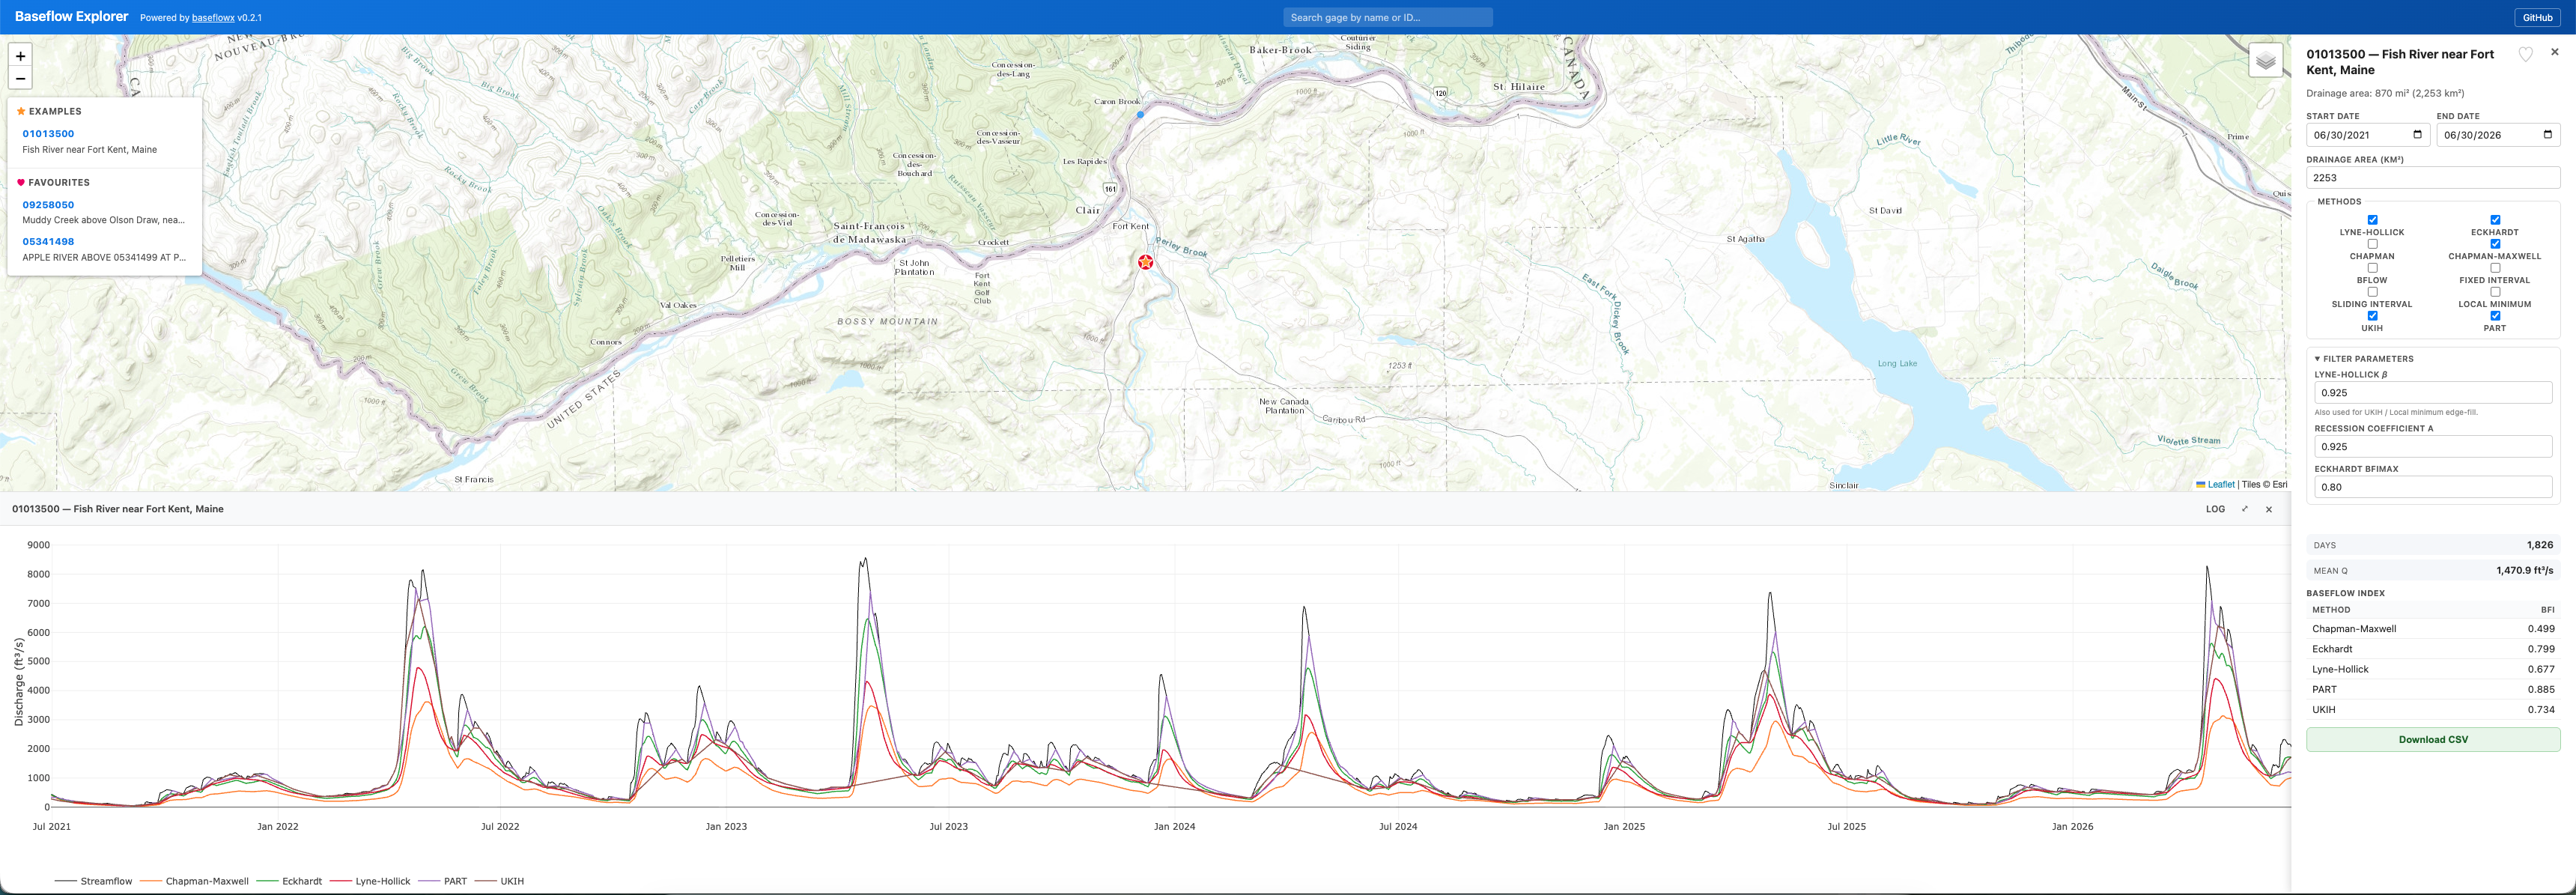
\includegraphics[width=\textwidth]{figures/baseflowx_web.png}
\caption{The Baseflow Explorer web application interface, showing the national stream gage map alongside the interactive hydrograph panel and multi-method BFI summary.\label{fig:webapp}}
\end{figure}

\subsection{Features and Interface}
\label{sec:webapp_features}

The application presents an interactive map displaying approximately 9{,}500 active USGS daily-values stream gages across the contiguous United States. Clicking any marker loads the station metadata and triggers an automatic baseflow analysis using default parameters. Key features include:

\begin{itemize}[nosep]
\item \textbf{Multi-method separation}: ten methods are available in the browser, spanning recursive digital filters (Lyne--Hollick, Eckhardt, Chapman, Chapman--Maxwell, BFlow) and graphical and recession-based methods (fixed interval, sliding interval, local minimum, UKIH, PART). Tracer-based CMB analysis is available in the Python library when concurrent specific conductance data are supplied.
\item \textbf{Interactive parameter adjustment}: filter parameters update the separation in real time; parameters that are not applicable to the active method are visually dimmed to guide the user toward method-appropriate inputs.
\item \textbf{Hydrograph visualization}: an interactive Plotly panel supports linear and logarithmic discharge axes, panel resizing, and full-screen mode, enabling visual inspection of both event-scale and seasonal baseflow dynamics.
\item \textbf{BFI summary table}: the application reports the baseflow index for each active method side by side, enabling rapid cross-method comparison without any scripting.
\item \textbf{CSV export}: the complete daily baseflow time series for all active methods can be downloaded for offline analysis or model calibration.
\item \textbf{Gage search, examples, and favorites}: a search box allows gages to be located by name or USGS site number; a curated example gage (01013500, Fish River near Fort Kent, Maine, the same station used throughout Sections~\ref{sec:examples} and~\ref{sec:validation}) is listed for one-click access, and users can save frequently analyzed gages to a persistent favorites list for quick recall in future sessions.
\end{itemize}

\subsection{Comparison with Existing Web Tools}
\label{sec:webapp_comparison}

The Baseflow Explorer builds on the concept established by the Web-based Hydrograph Analysis Tool (WHAT)~\cite{Lim2005} but extends it substantially in method coverage and data integration. WHAT supports three separation methods and requires manual upload of gage data; the Baseflow Explorer integrates directly with the USGS NWIS API and provides ten separation methods with live parameter adjustment and a national gage map. Compared with the USGS StreamStats web service, which focuses on flow statistics rather than hydrograph partitioning, the Baseflow Explorer is purpose-built for baseflow separation and cross-method comparison. The application therefore serves practitioners who need rapid exploratory analysis and educators who wish to demonstrate method sensitivity without configuring a Python environment, complementing the scripting capabilities of the \texttt{baseflowx} library.

%%%%%%%%%%%%%%%%%%%%%%%%%%%%%%%%%%%%%%%%%%
\section{Discussion}
\label{sec:discussion}

\subsection{Filter Family Taxonomy and Relationships}
\label{sec:taxonomy}

The generalized filter equation (Equation~\ref{eq:generalized}) provides a unifying lens through which to understand the relationships among recursive digital filters. Previous work has examined individual filter sensitivities~\cite{Kang2022}, but the unified framework presented here reveals structural connections across the full family of methods. Figure~\ref{fig:families} illustrates the structural difference between the two filter families during a peak flow event: the $\gamma = 0$ family (linear reservoir) responds only to the current streamflow, while the $\gamma = 1$ family (signal processing) incorporates a moving average of streamflow, producing different recession characteristics.

\begin{figure}[H]
\centering
\includegraphics[width=0.85\textwidth]{figures/filter_families.png}
\caption{Comparison of $\gamma = 0$ (linear reservoir) and $\gamma = 1$ (signal processing) filter families applied to a peak flow event, illustrating the structural difference in how each family partitions the hydrograph.\label{fig:families}}
\end{figure}

The IHACRES filter~\cite{Jakeman1993} occupies a unique position as a bridge between the two families. Its $\gamma = \alpha_s$ parameter allows continuous interpolation between the Boughton filter ($\alpha_s = 0$, pure $\gamma = 0$ behavior) and the signal-processing family ($\alpha_s \to -1$). Figure~\ref{fig:ihacres_sensitivity} demonstrates this transition, showing how the baseflow estimate varies as $\alpha_s$ changes from 0 to $-0.9$.

\begin{figure}[H]
\centering
\includegraphics[width=0.85\textwidth]{figures/ihacres_sensitivity.png}
\caption{Sensitivity of the IHACRES filter to the $\alpha_s$ parameter, showing the transition from $\gamma = 0$ family behavior ($\alpha_s = 0$, equivalent to Boughton) toward $\gamma = 1$ family behavior ($\alpha_s \to -1$).\label{fig:ihacres_sensitivity}}
\end{figure}

The algebraic equivalence between the Boughton and Eckhardt filters, related by $C = (1-a)\cdot\mathrm{BFI_{max}}/(1-\mathrm{BFI_{max}})$, means that the Eckhardt filter, parameterized in terms of the physically interpretable $\mathrm{BFI_{max}}$, subsumes both the Boughton and Chapman--Maxwell filters (the latter being the special case $\mathrm{BFI_{max}} = 0.5$).

\subsection{Comparison with Existing Tools}
\label{sec:comparison_tools}

Table~\ref{tab:comparison} summarizes how \texttt{baseflowx} and the Baseflow Explorer compare with the principal existing tools. As detailed in Section~\ref{sec:existing_tools}, prior tools were constrained by language barriers, limited method coverage, or lack of automation support. The \texttt{baseflowx} package addresses these gaps through 17 methods across all four paradigms in a single pip-installable library with integrated USGS data retrieval and a unified filter framework; the Baseflow Explorer extends access further by providing a web interface over the same analytical engine (Section~\ref{sec:webapp}). Together they cover the full range from batch scripting workflows to browser-based exploratory analysis, integrating naturally alongside established Python hydrology packages such as Hydrostats~\cite{Roberts2018} and Pastas~\cite{Collenteur2019}.

\begin{table}[H]
\caption{Comparison of \texttt{baseflowx} and the Baseflow Explorer with existing baseflow separation tools.\label{tab:comparison}}
\small
\begin{tabularx}{\textwidth}{lccccc}
\toprule
\textbf{Feature} & \textbf{baseflowx} & \textbf{Baseflow Explorer} & \textbf{HYSEP/PART} & \textbf{WHAT} & \textbf{baseflow}~\cite{Xie2020} \\
\midrule
Language / interface & Python & Web & Fortran & Web & Python \\
Methods & 17 & 10 & 4 & 3 & 11 \\
Scriptable/automatable & Yes & No & Limited & No & Yes \\
Tracer-based methods & Yes & No & No & No & No \\
USGS data retrieval & Yes & Yes & No & Yes & No \\
pip-installable & Yes & N/A & No & N/A & Yes \\
Active documentation & Yes & Yes & No & Yes & No \\
Unified filter framework & Yes & Yes & N/A & No & No \\
No-install access & No & Yes & No & Yes & No \\
\bottomrule
\end{tabularx}
\end{table}

\subsection{Limitations}
\label{sec:limitations}

Several limitations should be noted. First, the package currently operates on daily time-step data only; sub-daily applications (e.g., urban hydrology) or monthly aggregations would require adaptation of the filter equations and graphical method intervals. Second, all methods operate on single-station time series; spatial interpolation of baseflow across a watershed is not supported, though the scriptable API makes it straightforward to loop over multiple stations programmatically.

Third, the recursive digital filters are deterministic and do not provide uncertainty estimates. As shown in Table~\ref{tab:bfi}, different methods can yield BFI values that differ by 0.15 or more for the same record, and users should treat the spread across methods as a first-order uncertainty indicator rather than relying on any single estimate.

Fourth, for the CMB method, the assumption of two end-members and conservative mixing may not hold in all hydrogeological settings, particularly in catchments with multiple groundwater sources, evaporative concentration, or geochemical reactions that alter SC. Furthermore, as Zhang et al.~\cite{Zhang2021} demonstrated, calibrating Eckhardt filter parameters from CMB-derived baseflow works well at annual scales but can perform poorly at daily scales, and users should interpret daily-scale calibrated results with caution.

Finally, while the package includes parameter estimation tools, the recession coefficient and $\mathrm{BFI_{max}}$ estimates are sensitive to the period of record and the presence of regulation or diversions. Users working with regulated streams should exercise judgment in interpreting results.

\subsection{Future Development}
\label{sec:future}

Several directions for future development are planned. Support for sub-daily time steps would extend the package's applicability to urban and event-scale hydrology. Automated method selection algorithms could recommend appropriate methods based on catchment characteristics and data availability. Uncertainty quantification, either through bootstrap resampling or Bayesian parameter estimation, would provide formal confidence intervals on baseflow estimates. Integration of additional tracer types, such as stable isotopes~\cite{Klaus2013}, would expand the tracer module beyond conductivity. Finally, spatial baseflow mapping using gridded runoff data would support regional and continental-scale applications, building on the batch-processing capabilities that can be constructed from the existing single-station API.

%%%%%%%%%%%%%%%%%%%%%%%%%%%%%%%%%%%%%%%%%%
\section{Conclusions}
\label{sec:conclusions}

We have presented a review of baseflow separation methods spanning more than four decades of literature, and two open-source tools that make those methods accessible: the \texttt{baseflowx} Python package and the Baseflow Explorer web application. Together they cover four methodological paradigms (recursive digital filters, graphical methods, recession analysis, and tracer-based approaches), making 17 separation methods available from a pip-installable library or a browser interface over approximately 9{,}500 active USGS stream gages.

A key theoretical contribution is the identification of a generalized three-parameter recursive digital filter equation (Equation~\ref{eq:generalized}) that reveals the algebraic relationships among 11 popular methods, including the equivalence of the Boughton and Eckhardt filters and the bridging role of IHACRES between the two filter families. The package also provides the first Python implementation of the USGS PART method and a novel CMB-to-Eckhardt calibration bridge linking tracer measurements to digital filter parameters.

Both tools are designed for accessibility and reproducibility: \texttt{baseflowx} is pip-installable, provides built-in USGS data retrieval, includes bundled sample data, and is accompanied by comprehensive documentation; the Baseflow Explorer delivers the same analytical capability through a map-based web interface with live parameter adjustment and CSV export. We hope that these tools will serve hydrologists, water resource engineers, and educators, and that their open-source nature will foster community contributions and continued development.

%%%%%%%%%%%%%%%%%%%%%%%%%%%%%%%%%%%%%%%%%%
\vspace{6pt}

%%%%%%%%%%%%%%%%%%%%%%%%%%%%%%%%%%%%%%%%%%
%% optional
%\supplementary{The following supporting information can be downloaded at: \linksupplementary{s1}}

%%%%%%%%%%%%%%%%%%%%%%%%%%%%%%%%%%%%%%%%%%
\authorcontributions{Conceptualization, N.J. and T.P.C.; methodology, X.L. and A.A.; software, X.L., A.A., J.H., A.K. and B.B.; validation, X.L. and A.A.; writing---original draft preparation, X.L.; writing---review and editing, N.J., G.W., D.R. and T.P.C.; supervision, N.J. and T.P.C. All authors have read and agreed to the published version of the manuscript.}

\funding{This research received no external funding.}

%\informedconsent{}

\dataavailability{The \texttt{baseflowx} Python package is publicly available at \url{https://github.com/BYU-Hydroinformatics/baseflowx}. Documentation is available at \url{https://baseflowx.readthedocs.io/en/latest/}. The bundled sample dataset originates from USGS station 01013500 (Fish River near Fort Kent, Maine).}

\conflictsofinterest{The authors declare no conflicts of interest.}

%%%%%%%%%%%%%%%%%%%%%%%%%%%%%%%%%%%%%%%%%%
\begin{adjustwidth}{-\extralength}{0cm}

\reftitle{References}

\begin{thebibliography}{99}

\bibitem{Smakhtin2001}
Smakhtin, V.U. Low Flow Hydrology: A Review. \textit{J. Hydrol.} \textbf{2001}, \textit{240}, 147--186. \url{https://doi.org/10.1016/S0022-1694(00)00340-1}

\bibitem{Barlow2012}
Barlow, P.M.; Leake, S.A. Streamflow Depletion by Wells---Understanding and Managing the Effects of Groundwater Pumping on Streamflow; \textit{U.S. Geological Survey Circular 1376}; USGS: Reston, VA, USA, 2012; 84~p. \url{https://doi.org/10.3133/cir1376}

\bibitem{ChapmanMaxwell1996}
Chapman, T.G.; Maxwell, A.I. Baseflow Separation---Comparison of Numerical Methods with Tracer Experiments. In Proceedings of the Hydrology and Water Resources Symposium; Institution of Engineers Australia: Hobart, Australia, 1996; pp.~539--545.

\bibitem{Eckhardt2005}
Eckhardt, K. How to Construct Recursive Digital Filters for Baseflow Separation. \textit{Hydrol. Process.} \textbf{2005}, \textit{19}, 507--515. \url{https://doi.org/10.1002/hyp.5675}

\bibitem{Tan2020}
Tan, X.; Gan, T.Y. Global Changes in Baseflow Under the Impacts of Changing Climate and Vegetation. \textit{Water Resour. Res.} \textbf{2020}, \textit{56}, e2020WR027349. \url{https://doi.org/10.1029/2020WR027349}

\bibitem{Jasechko2024}
Jasechko, S.; Seybold, H.; Perrone, D.; et al. Rapid Groundwater Decline and Some Cases of Recovery in Aquifers Globally. \textit{Nature} \textbf{2024}, \textit{625}, 715--721. \url{https://doi.org/10.1038/s41586-023-06879-8}

\bibitem{Tallaksen1995}
Tallaksen, L.M. A Review of Baseflow Recession Analysis. \textit{J. Hydrol.} \textbf{1995}, \textit{165}, 349--370. \url{https://doi.org/10.1016/0022-1694(94)02540-R}

\bibitem{McMahon2021}
McMahon, T.A.; Nathan, R.J. Baseflow and Transmission Loss: A Review. \textit{WIREs Water} \textbf{2021}, \textit{8}, e1527. \url{https://doi.org/10.1002/wat2.1527}

\bibitem{Lyne1979}
Lyne, V.; Hollick, M. Stochastic Time-Variable Rainfall-Runoff Modelling. In Proceedings of the Hydrology and Water Resources Symposium; Institution of Engineers Australia: Perth, Australia, 1979; pp.~89--93.

\bibitem{Nathan1990}
Nathan, R.J.; McMahon, T.A. Evaluation of Automated Techniques for Base Flow and Recession Analyses. \textit{Water Resour. Res.} \textbf{1990}, \textit{26}, 1465--1473. \url{https://doi.org/10.1029/WR026i007p01465}

\bibitem{Chapman1991}
Chapman, T.G. Comment on ``Evaluation of Automated Techniques for Base Flow and Recession Analyses'' by R.~J.~Nathan and T.~A.~McMahon. \textit{Water Resour. Res.} \textbf{1991}, \textit{27}, 1783--1784. \url{https://doi.org/10.1029/91WR01007}

\bibitem{Sloto1996}
Sloto, R.A.; Crouse, M.Y. HYSEP: A Computer Program for Streamflow Hydrograph Separation and Analysis; \textit{U.S. Geological Survey Water-Resources Investigations Report 96-4040}; USGS: Lemoyne, PA, USA, 1996. \url{https://doi.org/10.3133/wri964040}

\bibitem{Rutledge1998}
Rutledge, A.T. Computer Programs for Describing the Recession of Ground-Water Discharge and for Estimating Mean Ground-Water Recharge and Discharge from Streamflow Records-Update; \textit{U.S. Geological Survey Water-Resources Investigations Report 98-4148}; USGS: Reston, VA, USA, 1998. \url{https://doi.org/10.3133/wri984148}

\bibitem{Stewart2007}
Stewart, M.T.; Cimino, J.; Ross, M. Calibration of Base Flow Separation Methods with Streamflow Conductivity. \textit{Groundwater} \textbf{2007}, \textit{45}, 17--27. \url{https://doi.org/10.1111/j.1745-6584.2006.00263.x}

\bibitem{Klaus2013}
Klaus, J.; McDonnell, J.J. Hydrograph Separation Using Stable Isotopes: Review and Evaluation. \textit{J. Hydrol.} \textbf{2013}, \textit{505}, 47--64. \url{https://doi.org/10.1016/j.jhydrol.2013.09.006}

\bibitem{Eckhardt2008}
Eckhardt, K. A Comparison of Baseflow Indices, Which Were Calculated with Seven Different Baseflow Separation Methods. \textit{J. Hydrol.} \textbf{2008}, \textit{352}, 168--173. \url{https://doi.org/10.1016/j.jhydrol.2008.01.005}

\bibitem{Lott2016}
Lott, D.A.; Stewart, M.T. Base Flow Separation: A Comparison of Analytical and Mass Balance Methods. \textit{J. Hydrol.} \textbf{2016}, \textit{535}, 525--533. \url{https://doi.org/10.1016/j.jhydrol.2016.01.063}

\bibitem{Lim2005}
Lim, K.J.; Engel, B.A.; Tang, Z.; Choi, J.; Kim, K.; Muthukrishnan, S.; Tripathy, D. Automated Web GIS Based Hydrograph Analysis Tool, WHAT. \textit{J. Am. Water Resour. Assoc.} \textbf{2005}, \textit{41}, 1407--1416. \url{https://doi.org/10.1111/j.1752-1688.2005.tb03808.x}

\bibitem{Pelletier2020}
Pelletier, A.; Andr\'{e}assian, V. Hydrograph Separation: An Impartial Parametrisation for an Imperfect Method. \textit{Hydrol. Earth Syst. Sci.} \textbf{2020}, \textit{24}, 1171--1187. \url{https://doi.org/10.5194/hess-24-1171-2020}

\bibitem{PelletierR2020}
Pelletier, A.; Andr\'{e}assian, V.; Delaigue, O. \textit{baseflow: Computes Hydrograph Separation}; R Package Version 1.3; INRAE: Paris, France, 2020. \url{https://doi.org/10.15454/Z9IK5N}

\bibitem{Xie2020}
Xie, J.; Liu, X.; Wang, K.; Yang, T.; Liang, K.; Liu, C. Evaluation of Typical Methods for Baseflow Separation in the Contiguous United States. \textit{J. Hydrol.} \textbf{2020}, \textit{583}, 124628. \url{https://doi.org/10.1016/j.jhydrol.2020.124628}

\bibitem{Roberts2018}
Roberts, W.; Williams, G.P.; Jackson, E.; Nelson, E.J.; Ames, D.P. Hydrostats: A Python Package for Characterizing Errors between Observed and Predicted Time Series. \textit{Hydrology} \textbf{2018}, \textit{5}, 66. \url{https://doi.org/10.3390/hydrology5040066}

\bibitem{Collenteur2019}
Collenteur, R.A.; Bakker, M.; Calje, R.; Klop, S.A.; Schaars, F. Pastas: Open Source Software for the Analysis of Groundwater Time Series. \textit{Groundwater} \textbf{2019}, \textit{57}, 877--885. \url{https://doi.org/10.1111/gwat.12925}

\bibitem{Barnes1939}
Barnes, B.S. The Structure of Discharge-Recession Curves. \textit{Trans. Am. Geophys. Union} \textbf{1939}, \textit{20}, 721--725.

\bibitem{Willems2009}
Willems, P. A Time Series Tool to Support the Multi-Criteria Performance Evaluation of Rainfall-Runoff Models. \textit{Environ. Model. Softw.} \textbf{2009}, \textit{24}, 311--321. \url{https://doi.org/10.1016/j.envsoft.2008.09.005}

\bibitem{Jakeman1993}
Jakeman, A.J.; Hornberger, G.M. How Much Complexity Is Warranted in a Rainfall-Runoff Model? \textit{Water Resour. Res.} \textbf{1993}, \textit{29}, 2637--2649. \url{https://doi.org/10.1029/93WR00877}

\bibitem{Arnold1999}
Arnold, J.G.; Allen, P.M. Automated Methods for Estimating Baseflow and Ground Water Recharge from Streamflow Records. \textit{J. Am. Water Resour. Assoc.} \textbf{1999}, \textit{35}, 411--424. \url{https://doi.org/10.1111/j.1752-1688.1999.tb03599.x}

\bibitem{Brutsaert1977}
Brutsaert, W.H.; Nieber, J.L. Regionalized Drought Flow Hydrographs from a Mature Glaciated Plateau. \textit{Water Resour. Res.} \textbf{1977}, \textit{13}, 637--643. \url{https://doi.org/10.1029/WR013i003p00637}

\bibitem{Cheng2016}
Cheng, L.; Zhang, L.; Brutsaert, W. Automated Selection of Pure Base Flows from Regular Daily Streamflow Data: Objective Algorithm. \textit{J. Hydrol. Eng.} \textbf{2016}, \textit{21}, 06016008. \url{https://doi.org/10.1061/(ASCE)HE.1943-5584.0001427}

\bibitem{Collischonn2013}
Collischonn, W.; Fan, F.M. Defining Parameters for Eckhardt's Digital Baseflow Filter. \textit{Hydrol. Process.} \textbf{2013}, \textit{27}, 2614--2622. \url{https://doi.org/10.1002/hyp.9391}

\bibitem{Boughton1993}
Boughton, W.C. A Hydrograph-Based Model for Estimating the Water Yield of Ungauged Catchments. In Proceedings of the Hydrology and Water Resources Symposium; Institution of Engineers Australia: Newcastle, Australia, 1993; pp.~317--324.

\bibitem{Tularam2008}
Tularam, G.A.; Ilahee, M. Exponential Smoothing Method of Base Flow Separation and Its Impact on Continuous Loss Estimates. \textit{Am. J. Environ. Sci.} \textbf{2008}, \textit{4}, 136--144. \url{https://doi.org/10.3844/ajessp.2008.136.144}

\bibitem{Furey2001}
Furey, P.R.; Gupta, V.K. A Physically Based Filter for Separating Base Flow from Streamflow Time Series. \textit{Water Resour. Res.} \textbf{2001}, \textit{37}, 2709--2722. \url{https://doi.org/10.1029/2001WR000243}

\bibitem{Spongberg2000}
Spongberg, M.E. Spectral Analysis of Base Flow Separation with Digital Filters. \textit{Water Resour. Res.} \textbf{2000}, \textit{36}, 745--752. \url{https://doi.org/10.1029/1999WR900303}

\bibitem{UKIH1980}
Institute of Hydrology. \textit{Low Flow Studies Report No. 1}; Institute of Hydrology: Wallingford, UK, 1980. \url{https://nora.nerc.ac.uk/id/eprint/9093}

\bibitem{Wittenberg1999}
Wittenberg, H.; Sivapalan, M. Watershed Groundwater Balance Estimation Using Streamflow Recession Analysis and Baseflow Separation. \textit{J. Hydrol.} \textbf{1999}, \textit{219}, 20--33. \url{https://doi.org/10.1016/S0022-1694(99)00040-2}

\bibitem{Miller2015}
Miller, M.P.; Johnson, H.M.; Susong, D.D.; Wolock, D.M. A New Approach for Continuous Estimation of Baseflow Using Discrete Water Quality Data: Method Description and Comparison with Baseflow Estimates from Two Existing Approaches. \textit{J. Hydrol.} \textbf{2015}, \textit{522}, 203--210. \url{https://doi.org/10.1016/j.jhydrol.2014.12.039}

\bibitem{Zhang2021}
Zhang, J.; Song, J.; Cheng, L.; Zheng, H.; Wang, Y.; Huai, B.; Sun, W.; Qi, S.; Zhao, P.; Wang, Y.; Li, Q. Can the Two-Parameter Recursive Digital Filter Really Be Calibrated by the Conductivity Mass Balance Method? \textit{Hydrol. Earth Syst. Sci.} \textbf{2021}, \textit{25}, 1747--1760. \url{https://doi.org/10.5194/hess-25-1747-2021}

\bibitem{Harris2020}
Harris, C.R.; Millman, K.J.; van~der~Walt, S.J.; Gommers, R.; Virtanen, P.; Cournapeau, D.; Wieser, E.; Taylor, J.; Berg, S.; Smith, N.J.; et~al. Array Programming with NumPy. \textit{Nature} \textbf{2020}, \textit{585}, 357--362. \url{https://doi.org/10.1038/s41586-020-2649-2}

\bibitem{McKinney2010}
McKinney, W. Data Structures for Statistical Computing in Python. In Proceedings of the 9th Python in Science Conference; Austin, TX, USA, 2010; pp.~56--61. \url{https://doi.org/10.25080/Majora-92bf1922-00a}

\bibitem{Lam2015}
Lam, S.K.; Pitrou, A.; Seibert, S. Numba: A LLVM-Based Python JIT Compiler. In Proceedings of the Second Workshop on the LLVM Compiler Infrastructure in HPC (LLVM '15); ACM: New York, NY, USA, 2015; pp.~1--6. \url{https://doi.org/10.1145/2833157.2833162}

\bibitem{BaseflowxDocs}
baseflowx Documentation. Available online: \url{https://baseflowx.readthedocs.io/en/latest/} (accessed on 26 June 2026).

\bibitem{Kang2022}
Kang, T.; Lee, S.; Lee, N.; Jin, Y. Baseflow Separation Using the Digital Filter Method: Review and Sensitivity Analysis. \textit{Water} \textbf{2022}, \textit{14}, 485. \url{https://doi.org/10.3390/w14030485}

\bibitem{Bloomfield2009}
Bloomfield, J.P.; Allen, D.J.; Griffiths, K.J. Examining Geological Controls on Baseflow Index (BFI) Using Regression Analysis: An Illustration from the Thames Basin, UK. \textit{J. Hydrol.} \textbf{2009}, \textit{373}, 164--176. \url{https://doi.org/10.1016/j.jhydrol.2009.04.025}

\bibitem{Santhi2008}
Santhi, C.; Allen, P.M.; Muttiah, R.S.; Arnold, J.G.; Tuppad, P. Regional Estimation of Base Flow for the Conterminous United States by Hydrologic Landscape Regions. \textit{J. Hydrol.} \textbf{2008}, \textit{351}, 139--153. \url{https://doi.org/10.1016/j.jhydrol.2007.12.018}

\bibitem{Neff2005}
Neff, B.P.; Day, S.M.; Piggott, A.R.; Fuller, L.M. \textit{Baseflow in the Great Lakes Basin}; U.S. Geological Survey Scientific Investigations Report 2005-5217; USGS: Reston, VA, USA, 2005. \url{https://doi.org/10.3133/sir20055217}

\end{thebibliography}

\end{adjustwidth}

\end{document}
